\documentclass{article}
\usepackage[utf8]{inputenc}
\usepackage{fullpage,amsmath,hyperref,indentfirst,graphicx,wrapfig,caption,subcaption}
\graphicspath{{~/Desktop/JUPYTER-LAB}}
\date{}
\begin{document}
{\LARGE{\hskip 2.2 in CS170 Project 1}}
\vskip 0.5in
{\flushleft{Brandon Paulsen}}
{\flushleft{October 31$^\text{st}$, 2022}}
{\flushleft{UCR CS170 Fall 2022}}
{\flushleft{Professor Eamonn Keough}}
\vskip 0.5in
\tableofcontents
\listoffigures
\pagebreak
\section{Introduction}
In this project, we are asked to write a program that uses a general search algorithm (A*) to solve 8 puzzles. An 8 puzzle is a puzzle that has 8 tiles arranged in a 3x3 grid, with one space. The goal of the puzzle is to arrange the tiles such that the first row is [1,2,3], the second row is [4,5,6], and the last row is [7,8,empty] by moving tiles around. Tiles next to the empty tile can swap places with the empty tile, or we can understand this as the empty tile swapping with tiles next to it.
\par A* is a search agorithm that uses both the depth of a state and a heuristic function to gague which unexplored states in the frontier should be explored first. It does this by assigning each state in the frontier a priority that is equal to the sum of the depth and heuristic, and as long as the heuristic is admissible (that is, it never overestimates the number of moves from the state to the goal state), A* will be optimal. In this project, we are tasked with implementing 3 heuristic functions: Uniform Cost, Misplaced Tiles, and Manhattan Distance.
\par As has been discussed in class multiple times, the branching factor and diameter of a search problem are very important. In fact, the branching factor and the problem diameter of a search problem define the magnitude of the search space, so it might be good to investigate them a little bit. Based on the loose idea that the branching factor is the average of the number of valid moves of a state, we can approximate the branching factor as $4\cdot\frac{1}{9}+3\cdot\frac{4}{9}+2\cdot\frac{4}{9} = \frac{24}{9} \approx 2.6$, because there are 4 corner spaces with 2 moves, 4 edge spaces with 3 moves, and 1 center space with 4 moves. This seems reasonable, but if we further consider that we cannot go back to any states previously visited, and at least one move for each state goes back to a previous state, we can reduce the approximate branching factor to $3\cdot\frac{1}{9}+2\cdot\frac{4}{9}+1\cdot\frac{4}{9} = \frac{15}{9} \approx 1.7$. This is a very small branching factor, which is great news for us. We can further extend this approximation of the branching factor to any n puzzle as $\frac{4}{n^2}+\frac{8\cdot(n-2)}{n^2}+\frac{3\cdot(n^2-4\cdot(n-2)-4)}{n^2} = 3-\frac{4}{n}$.
\section{Heuristics}
Heuristics are a the heart of the A* algorithm, without them, A* would be no better than breadth first search. As such, it is important to discuss the heuristics used in this project both in terms of their implementation and their impact on space and time complexity.
\subsection{Uniform Cost}
Uniform Cost Heuristic is the simplest of the 3 heuristics. It simply evaluates to 0 for all states. This means that in effect, A* with Uniform Cost Heuristic devolves to breadth first search and searches level-by-level. This clearly implies that the algorithm will be complete and optimal, though it will be very slow and memory inefficient as well.
\subsection{Misplaced Tile}
Misplaced Tile Heuristic, though slightly more complex than Uniform Cost Heuristic (which is trivial), is not overly complex. Evaluating the Misplaced Tile Heuristic of a state amounts to counting up the number of tiles in a given state that are not in the same position as they are in the goal state. Though it is much better than Uniform Cost Heuristic, it is clearly not the best heuristic (either in terms of time or memory), as children of a state (those states that are reachable from that state in a move) often are assigned the same priority, and therefore the search algorithm has a hard time distinguishing which is better and should be explored first.
\subsection{Manhattan Distance}
Though Manhattan Distance Heuristic is the most complex of the 3, it offers some potential benefits that warrant its use. In all cases, Manhattan Distance Heuristic dominates Misplaced Tile Heuristic - that is to say, its value is greater than Misplaced Tile Hueristic without overestimating the number of moves left and therefore destroying the optimality of the A* algorithm. The Manhattan Distance Heuristic is calculated by totaling the differences in x and y positions of tiles between a given state and the goal state, or in math terms, $\sum_{\text{tiles}\neq\text{empty}}\Delta x + \Delta y$. Though Manhattan Distance Heuristic is admissible, it is clearly not perfect, and there is still room for improvement.
\section{Test Cases}
Several cases were given in the project assignment. They range from trivial (depth 0) to very complex (depth 24) and make for good tests of algorithms. For a significant portion of time, my implementation of the general search algorithm when used with Manhattan Distance Heuristic failed to find the most optimal path (the path it found was at depth 26). This was very helpful to me in that it indicated an error in my code. The number of vistied nodes, frontier nodes, and searh time trends are plotted below for each heuristic:
\begin{figure}[ht]
	\centering
	\begin{subfigure}[b]{0.32\textwidth}
		\centering
		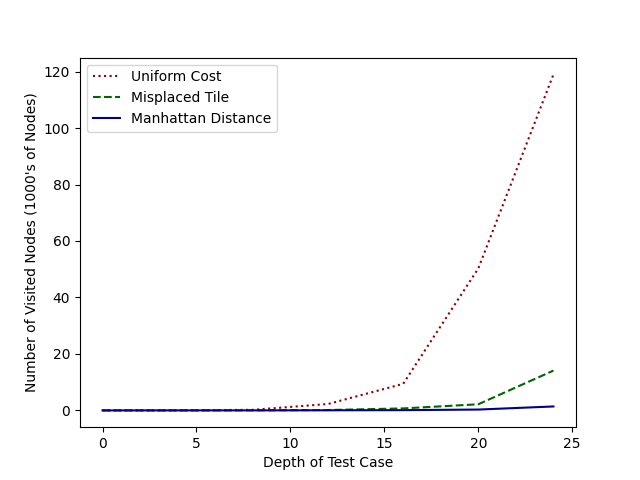
\includegraphics[width = \textwidth]{testVisitedComparison.png}
		\caption{Visited Nodes vs Depth}
		\label{fig:Test Visited Nodes Comparison}
	\end{subfigure}
	\hfill
	\begin{subfigure}[b]{0.32\textwidth}
		\centering
		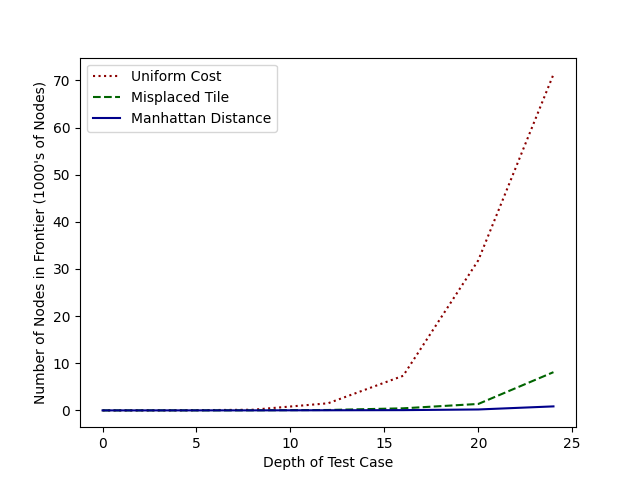
\includegraphics[width = \textwidth]{testFrontierComparison.png}
		\caption{Maximum Frontier Size vs Depth}
		\label{fig:Test Maximum Frontier Size Comparison}
	\end{subfigure}
	\hfill
	\begin{subfigure}[b]{0.32\textwidth}
		\centering
		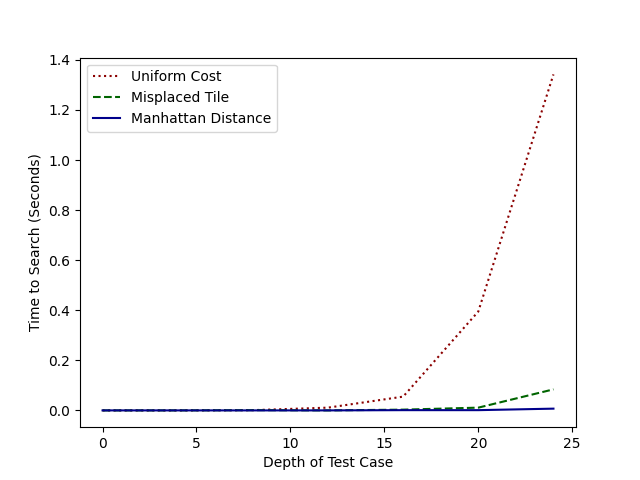
\includegraphics[width = \textwidth]{testTimeComparison.png}
		\caption{Search Time vs Depth}
		\label{fig:Test Search Time Comparison}
	\end{subfigure}
	\caption{Test Cases Trend Comparisons}
	\label{fig:Test Cases Trend Comparisons}
\end{figure}
\par As we can see quite clearly in the plots in Figure \ref{fig:Test Cases Trend Comparisons}, Uniform Cost performs significantly worse than either of the other heuristics over the test cases in terms of the visited nodes, maximum frontier size, and search time. Misplaced Tile performs slightly better, though still worse than Manhattan Distance. It is important to note that though these plots seem to indicate that Manhattan Distance is linear in the number of visited nodes, maximum frontier size, and search time, it is very much still exponential (as seen in Figures \ref{fig:Monte Carlo Visited Nodes Comparison} and \ref{fig:Monte Carlo Maximum Frontier Size Comparison}), though it grows much much slower than uniform cost.
\section{Monte Carlo Simulation}
I ran a monte carlo simulation on $10\%$ of the number of solvable states of the 8 puzzle (so, $\frac{9!}{20} = 18,144$ simulations) on each of the heuristics in order to see the trends of these heuristics beyond the test cases. It is probably overkill to run such a simulation, but I just had to satisfy my curiousity. All results of the monte carlo simulation have been plotted using python and included below. Below are plotted trend comparisons for the number of visited ndoes, the number of nodes in the frontier, and the search time vs depth for each heuristic:
\begin{figure}[ht]
	\centering
	\begin{subfigure}[b]{0.32\textwidth}
		\centering
		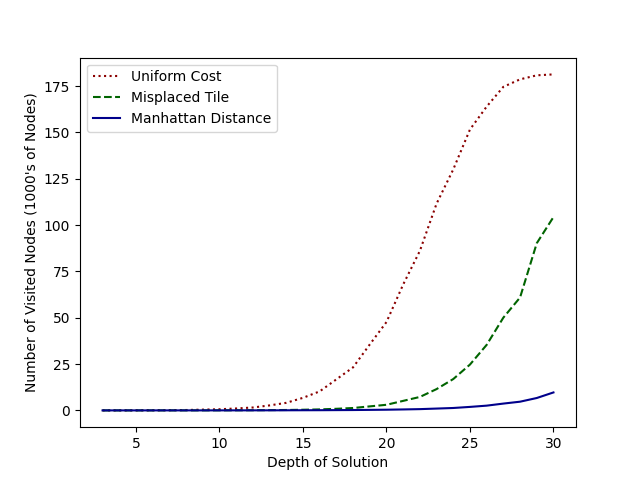
\includegraphics[width = \textwidth]{visitedComparison.png}
		\caption{Visited Nodes vs Depth}
		\label{fig:Monte Carlo Visited Nodes Comparison}
	\end{subfigure}
	\hfill
	\begin{subfigure}[b]{0.32\textwidth}
		\centering
		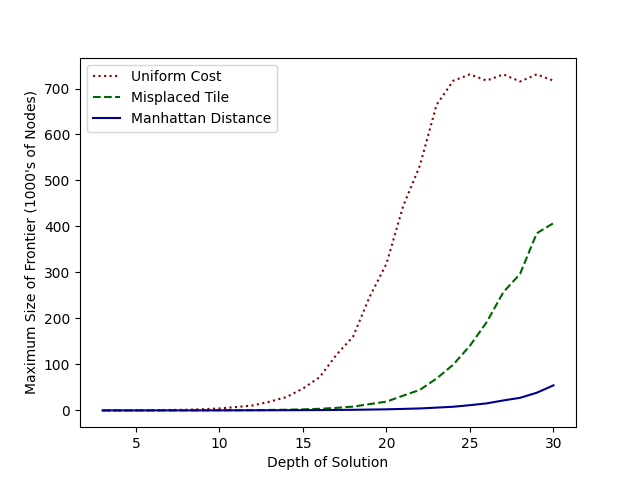
\includegraphics[width = \textwidth]{frontierComparison.png}
		\caption{Maximum Frontier Size vs Depth}
		\label{fig:Monte Carlo Maximum Frontier Size Comparison}
	\end{subfigure}
	\hfill
	\begin{subfigure}[b]{0.32\textwidth}
		\centering
		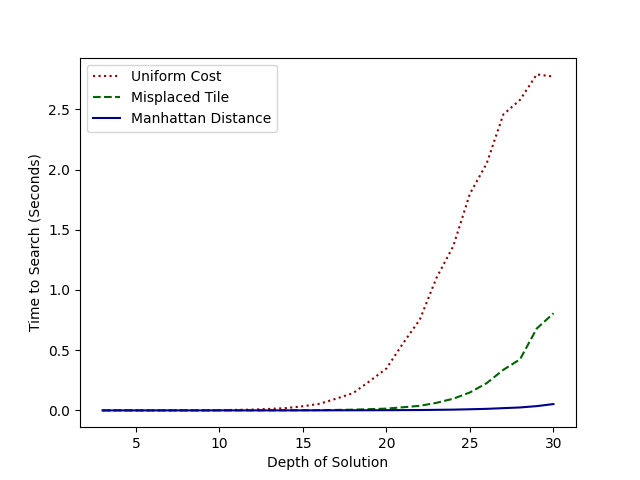
\includegraphics[width = \textwidth]{timeComparison.png}
		\caption{Search Time vs Depth}
		\label{fig:Monte Carlo Search Time Comparison}
	\end{subfigure}
	\caption{Monte Carlo Simulation Trend Comparisons}
	\label{fig:Monte Carlo Trend Comparisons}
\end{figure}
\pagebreak
\par In the Monte Carlo simulation, we observe many of the same trends as in the test cases. Uniform Cost search is still much more inefficient in all regards, while Manhattan Distance is stil the fastest. Now, however, in Figures \ref{fig:Monte Carlo Visited Nodes Comparison} and \ref{fig:Monte Carlo Maximum Frontier Size Comparison}, all heuristics are clearly nonlinear, whereas in the test cases, it appeared as though they were.
\section{Conclusion}
In conclusion, through this project, we have seen that each heuristic is optimal and complete, though they vary in their runtimes and memory complexity. Each heuristic is exponential with respect to its time and space complexity, though the Manhattan Distance is clearly much faster and uses much less memory on average than the other two (as can be seen in Figure \ref{fig:Search Time Comparison} and Figure \ref{fig:Frontier Comparison}, respectively).
\par Though the code is capable of solving 15 puzzles currently (the object based C++ version), it takes somewhere on the order of 5-10 minutes, so I would want to modify it to implement island based search.  I would expect this to significantly speed up the search (though it would no longer be optimal), possibly to something on the order of 30-50 seconds.
\section{Code}
\subsection{C++}
My object based C++ code (slower but more memory efficient) can be found at \url{https://github.com/Poly1581/SlidingPuzzlesV2}. My pointer based C++ code (slightly faster but much uglier and more memory inefficient) can be found at \url{https://github.com/Poly1581/SlidingPuzzles}
\subsection{Python}
My python code can be found at \url{https://github.com/Poly1581/PYSlidingPuzzles}
\section{References}
In the process of streamlining the randomization function in my object oriented code, I referenced the wikipedia page for the 15 puzzle to get a better understanding of the parity argument that allows for discrimination between solvable and unsolvable states. The page can be found here: \url{https://en.wikipedia.org/wiki/15_puzzle}.
\section{Example Trace of a Simple 8 Puzzle (Manhattan Distance)}
{\noindent What size puzzle would you like to solve?\newline}
3
What heuristic would you like to use?\newline
1:	Uniform Cost\newline
2:	Misplaced Tile\newline
3:	Manhattan Distance\newline
3
Would you like to use your own matrix or a random one?\newline
1:	User matrix\newline
2:	Random matrix\newline
1
Enter tile at row 0, and col 0\newline
1
Enter tile at row 0, and col 1\newline
2
Enter tile at row 0, and col 2\newline
3
Enter tile at row 1, and col 0\newline
5
Enter tile at row 1, and col 1\newline
0
Enter tile at row 1, and col 2\newline
6
Enter tile at row 2, and col 0\newline
4
Enter tile at row 2, and col 1\newline
7
Enter tile at row 2, and col 2\newline
8
{\noindent Best state to expand with depth (g(n)) 0 and heuristic (h(n)) 0\newline}
{\noindent 1\textbar 2\textbar 3}\newline
5\textbar 0\textbar 6\newline
4\textbar 7\textbar 8\newline

{\noindent Best state to expand with depth (g(n)) 1 and heuristic (h(n)) 3\newline}
{\noindent 1\textbar 2\textbar 3}\newline
0\textbar 5\textbar 6\newline
4\textbar 7\textbar 8\newline

{\noindent Best state to expand with depth (g(n)) 2 and heuristic (h(n)) 2\newline}
{\noindent 1\textbar 2\textbar 3}\newline
4\textbar 5\textbar 6\newline
0\textbar 7\textbar 8\newline

{\noindent Best state to expand with depth (g(n)) 3 and heuristic (h(n)) 1\newline}
{\noindent 1\textbar 2\textbar 3}\newline
4\textbar 5\textbar 6\newline
7\textbar 0\textbar 8\newline

{\noindent Best state to expand with depth (g(n)) 4 and heuristic (h(n)) 0\newline}
{\noindent 1\textbar 2\textbar 3}\newline
4\textbar 5\textbar 6\newline
7\textbar 8\textbar 0\newline

{\noindent Solution found\newline}
Path\newline
{\noindent 1\textbar 2\textbar 3}\newline
5\textbar 0\textbar 6\newline
4\textbar 7\textbar 8\newline

{\noindent 1\textbar 2\textbar 3}\newline
0\textbar 5\textbar 6\newline
4\textbar 7\textbar 8\newline

{\noindent 1\textbar 2\textbar 3}\newline
4\textbar 5\textbar 6\newline
0\textbar 7\textbar 8\newline

{\noindent 1\textbar 2\textbar 3}\newline
4\textbar 5\textbar 6\newline
7\textbar 0\textbar 8\newline

{\noindent 1\textbar 2\textbar 3}\newline
4\textbar 5\textbar 6\newline
7\textbar 8\textbar 0\newline

{\noindent Depth of solution 4\newline}
Number of visited nodes 5\newline
Max frontier size 5\newline
Search took 0 milliseconds\newline
\section{Example Trace of a Difficult 8 Puzzle (Manhattan Distance)}
{\noindent What size puzzle would you like to solve?\newline}
3
What heuristic would you like to use?\newline
1:	Uniform Cost\newline
2:	Misplaced Tile\newline
3:	Manhattan Distance\newline
3
Would you like to use your own matrix or a random one?\newline
1:	User matrix\newline
2:	Random matrix\newline
1
Enter tile at row 0, and col 0\newline
1
Enter tile at row 0, and col 1\newline
6
Enter tile at row 0, and col 2\newline
7
Enter tile at row 1, and col 0\newline
5
Enter tile at row 1, and col 1\newline
0
Enter tile at row 1, and col 2\newline
3
Enter tile at row 2, and col 0\newline
4
Enter tile at row 2, and col 1\newline
8
Enter tile at row 2, and col 2\newline
2
{\noindent Best state to expand with depth (g(n)) 0 and heuristic (h(n)) 0\newline}
{\noindent 1\textbar 6\textbar 7}\newline
5\textbar 0\textbar 3\newline
4\textbar 8\textbar 2\newline

{\noindent Best state to expand with depth (g(n)) 1 and heuristic (h(n)) 11\newline}
{\noindent 1\textbar 0\textbar 7}\newline
5\textbar 6\textbar 3\newline
4\textbar 8\textbar 2\newline

{\noindent Best state to expand with depth (g(n)) 1 and heuristic (h(n)) 11\newline}
{\noindent 1\textbar 6\textbar 7}\newline
0\textbar 5\textbar 3\newline
4\textbar 8\textbar 2\newline

{\noindent Best state to expand with depth (g(n)) 2 and heuristic (h(n)) 10\newline}
{\noindent 1\textbar 7\textbar 0}\newline
5\textbar 6\textbar 3\newline
4\textbar 8\textbar 2\newline

{\noindent Best state to expand with depth (g(n)) 2 and heuristic (h(n)) 10\newline}
{\noindent 1\textbar 6\textbar 7}\newline
4\textbar 5\textbar 3\newline
0\textbar 8\textbar 2\newline

{\noindent Best state to expand with depth (g(n)) 3 and heuristic (h(n)) 9\newline}
{\noindent 1\textbar 7\textbar 3}\newline
5\textbar 6\textbar 0\newline
4\textbar 8\textbar 2\newline

{\noindent Best state to expand with depth (g(n)) 4 and heuristic (h(n)) 8\newline}
{\noindent 1\textbar 7\textbar 3}\newline
5\textbar 6\textbar 2\newline
4\textbar 8\textbar 0\newline

{\noindent Best state to expand with depth (g(n)) 4 and heuristic (h(n)) 8\newline}
{\noindent 1\textbar 7\textbar 3}\newline
5\textbar 0\textbar 6\newline
4\textbar 8\textbar 2\newline

{\noindent Best state to expand with depth (g(n)) 5 and heuristic (h(n)) 7\newline}
{\noindent 1\textbar 0\textbar 3}\newline
5\textbar 7\textbar 6\newline
4\textbar 8\textbar 2\newline

{\noindent Best state to expand with depth (g(n)) 5 and heuristic (h(n)) 7\newline}
{\noindent 1\textbar 7\textbar 3}\newline
0\textbar 5\textbar 6\newline
4\textbar 8\textbar 2\newline

{\noindent Best state to expand with depth (g(n)) 6 and heuristic (h(n)) 6\newline}
{\noindent 1\textbar 7\textbar 3}\newline
4\textbar 5\textbar 6\newline
0\textbar 8\textbar 2\newline

{\noindent Best state to expand with depth (g(n)) 1 and heuristic (h(n)) 13\newline}
{\noindent 1\textbar 6\textbar 7}\newline
5\textbar 3\textbar 0\newline
4\textbar 8\textbar 2\newline

{\noindent Best state to expand with depth (g(n)) 6 and heuristic (h(n)) 8\newline}
{\noindent 0\textbar 1\textbar 3}\newline
5\textbar 7\textbar 6\newline
4\textbar 8\textbar 2\newline

{\noindent Best state to expand with depth (g(n)) 2 and heuristic (h(n)) 12\newline}
{\noindent 0\textbar 1\textbar 7}\newline
5\textbar 6\textbar 3\newline
4\textbar 8\textbar 2\newline

{\noindent Best state to expand with depth (g(n)) 7 and heuristic (h(n)) 7\newline}
{\noindent 1\textbar 7\textbar 3}\newline
4\textbar 5\textbar 6\newline
8\textbar 0\textbar 2\newline

{\noindent Best state to expand with depth (g(n)) 2 and heuristic (h(n)) 12\newline}
{\noindent 1\textbar 6\textbar 7}\newline
5\textbar 3\textbar 2\newline
4\textbar 8\textbar 0\newline

{\noindent Best state to expand with depth (g(n)) 5 and heuristic (h(n)) 9\newline}
{\noindent 1\textbar 7\textbar 3}\newline
5\textbar 6\textbar 2\newline
4\textbar 0\textbar 8\newline

{\noindent Best state to expand with depth (g(n)) 8 and heuristic (h(n)) 6\newline}
{\noindent 1\textbar 7\textbar 3}\newline
4\textbar 5\textbar 6\newline
8\textbar 2\textbar 0\newline

{\noindent Best state to expand with depth (g(n)) 3 and heuristic (h(n)) 11\newline}
{\noindent 1\textbar 6\textbar 7}\newline
4\textbar 5\textbar 3\newline
8\textbar 0\textbar 2\newline

{\noindent Best state to expand with depth (g(n)) 2 and heuristic (h(n)) 12\newline}
{\noindent 0\textbar 6\textbar 7}\newline
1\textbar 5\textbar 3\newline
4\textbar 8\textbar 2\newline

{\noindent Best state to expand with depth (g(n)) 4 and heuristic (h(n)) 10\newline}
{\noindent 1\textbar 6\textbar 7}\newline
4\textbar 5\textbar 3\newline
8\textbar 2\textbar 0\newline

{\noindent Best state to expand with depth (g(n)) 2 and heuristic (h(n)) 12\newline}
{\noindent 1\textbar 6\textbar 0}\newline
5\textbar 3\textbar 7\newline
4\textbar 8\textbar 2\newline

{\noindent Best state to expand with depth (g(n)) 6 and heuristic (h(n)) 8\newline}
{\noindent 0\textbar 7\textbar 3}\newline
1\textbar 5\textbar 6\newline
4\textbar 8\textbar 2\newline

{\noindent Best state to expand with depth (g(n)) 3 and heuristic (h(n)) 11\newline}
{\noindent 1\textbar 0\textbar 6}\newline
5\textbar 3\textbar 7\newline
4\textbar 8\textbar 2\newline

{\noindent Best state to expand with depth (g(n)) 7 and heuristic (h(n)) 7\newline}
{\noindent 7\textbar 0\textbar 3}\newline
1\textbar 5\textbar 6\newline
4\textbar 8\textbar 2\newline

{\noindent Best state to expand with depth (g(n)) 4 and heuristic (h(n)) 10\newline}
{\noindent 1\textbar 3\textbar 6}\newline
5\textbar 0\textbar 7\newline
4\textbar 8\textbar 2\newline

{\noindent Best state to expand with depth (g(n)) 1 and heuristic (h(n)) 13\newline}
{\noindent 1\textbar 6\textbar 7}\newline
5\textbar 8\textbar 3\newline
4\textbar 0\textbar 2\newline

{\noindent Best state to expand with depth (g(n)) 6 and heuristic (h(n)) 8\newline}
{\noindent 1\textbar 3\textbar 0}\newline
5\textbar 7\textbar 6\newline
4\textbar 8\textbar 2\newline

{\noindent Best state to expand with depth (g(n)) 5 and heuristic (h(n)) 9\newline}
{\noindent 1\textbar 7\textbar 3}\newline
5\textbar 8\textbar 6\newline
4\textbar 0\textbar 2\newline

{\noindent Best state to expand with depth (g(n)) 5 and heuristic (h(n)) 9\newline}
{\noindent 1\textbar 3\textbar 6}\newline
5\textbar 7\textbar 0\newline
4\textbar 8\textbar 2\newline

{\noindent Best state to expand with depth (g(n)) 5 and heuristic (h(n)) 9\newline}
{\noindent 1\textbar 3\textbar 6}\newline
0\textbar 5\textbar 7\newline
4\textbar 8\textbar 2\newline

{\noindent Best state to expand with depth (g(n)) 6 and heuristic (h(n)) 8\newline}
{\noindent 1\textbar 7\textbar 3}\newline
5\textbar 8\textbar 6\newline
4\textbar 2\textbar 0\newline

{\noindent Best state to expand with depth (g(n)) 6 and heuristic (h(n)) 8\newline}
{\noindent 1\textbar 3\textbar 6}\newline
5\textbar 7\textbar 2\newline
4\textbar 8\textbar 0\newline

{\noindent Best state to expand with depth (g(n)) 6 and heuristic (h(n)) 8\newline}
{\noindent 1\textbar 3\textbar 6}\newline
4\textbar 5\textbar 7\newline
0\textbar 8\textbar 2\newline

{\noindent Best state to expand with depth (g(n)) 2 and heuristic (h(n)) 12\newline}
{\noindent 1\textbar 6\textbar 7}\newline
5\textbar 8\textbar 3\newline
4\textbar 2\textbar 0\newline

{\noindent Best state to expand with depth (g(n)) 7 and heuristic (h(n)) 9\newline}
{\noindent 5\textbar 1\textbar 3}\newline
0\textbar 7\textbar 6\newline
4\textbar 8\textbar 2\newline

{\noindent Best state to expand with depth (g(n)) 4 and heuristic (h(n)) 12\newline}
{\noindent 1\textbar 6\textbar 7}\newline
4\textbar 0\textbar 3\newline
8\textbar 5\textbar 2\newline

{\noindent Best state to expand with depth (g(n)) 4 and heuristic (h(n)) 12\newline}
{\noindent 0\textbar 1\textbar 6}\newline
5\textbar 3\textbar 7\newline
4\textbar 8\textbar 2\newline

{\noindent Best state to expand with depth (g(n)) 7 and heuristic (h(n)) 9\newline}
{\noindent 1\textbar 3\textbar 6}\newline
4\textbar 5\textbar 7\newline
8\textbar 0\textbar 2\newline

{\noindent Best state to expand with depth (g(n)) 3 and heuristic (h(n)) 13\newline}
{\noindent 1\textbar 6\textbar 7}\newline
5\textbar 8\textbar 0\newline
4\textbar 2\textbar 3\newline

{\noindent Best state to expand with depth (g(n)) 8 and heuristic (h(n)) 8\newline}
{\noindent 5\textbar 1\textbar 3}\newline
7\textbar 0\textbar 6\newline
4\textbar 8\textbar 2\newline

{\noindent Best state to expand with depth (g(n)) 3 and heuristic (h(n)) 13\newline}
{\noindent 1\textbar 6\textbar 7}\newline
5\textbar 3\textbar 2\newline
4\textbar 0\textbar 8\newline

{\noindent Best state to expand with depth (g(n)) 8 and heuristic (h(n)) 8\newline}
{\noindent 1\textbar 3\textbar 6}\newline
4\textbar 5\textbar 7\newline
8\textbar 2\textbar 0\newline

{\noindent Best state to expand with depth (g(n)) 8 and heuristic (h(n)) 8\newline}
{\noindent 1\textbar 7\textbar 3}\newline
4\textbar 0\textbar 6\newline
8\textbar 5\textbar 2\newline

{\noindent Best state to expand with depth (g(n)) 6 and heuristic (h(n)) 10\newline}
{\noindent 1\textbar 7\textbar 3}\newline
5\textbar 0\textbar 2\newline
4\textbar 6\textbar 8\newline

{\noindent Best state to expand with depth (g(n)) 9 and heuristic (h(n)) 7\newline}
{\noindent 1\textbar 3\textbar 6}\newline
4\textbar 5\textbar 0\newline
8\textbar 2\textbar 7\newline

{\noindent Best state to expand with depth (g(n)) 9 and heuristic (h(n)) 7\newline}
{\noindent 1\textbar 0\textbar 3}\newline
4\textbar 7\textbar 6\newline
8\textbar 5\textbar 2\newline

{\noindent Best state to expand with depth (g(n)) 4 and heuristic (h(n)) 12\newline}
{\noindent 1\textbar 6\textbar 0}\newline
5\textbar 8\textbar 7\newline
4\textbar 2\textbar 3\newline

{\noindent Best state to expand with depth (g(n)) 3 and heuristic (h(n)) 13\newline}
{\noindent 5\textbar 1\textbar 7}\newline
0\textbar 6\textbar 3\newline
4\textbar 8\textbar 2\newline

{\noindent Best state to expand with depth (g(n)) 7 and heuristic (h(n)) 9\newline}
{\noindent 1\textbar 7\textbar 3}\newline
0\textbar 5\textbar 2\newline
4\textbar 6\textbar 8\newline

{\noindent Best state to expand with depth (g(n)) 5 and heuristic (h(n)) 11\newline}
{\noindent 1\textbar 0\textbar 6}\newline
5\textbar 8\textbar 7\newline
4\textbar 2\textbar 3\newline

{\noindent Best state to expand with depth (g(n)) 6 and heuristic (h(n)) 10\newline}
{\noindent 1\textbar 7\textbar 3}\newline
5\textbar 8\textbar 6\newline
0\textbar 4\textbar 2\newline

{\noindent Best state to expand with depth (g(n)) 6 and heuristic (h(n)) 10\newline}
{\noindent 1\textbar 7\textbar 3}\newline
5\textbar 6\textbar 2\newline
0\textbar 4\textbar 8\newline

{\noindent Best state to expand with depth (g(n)) 7 and heuristic (h(n)) 9\newline}
{\noindent 1\textbar 3\textbar 6}\newline
5\textbar 7\textbar 2\newline
4\textbar 0\textbar 8\newline

{\noindent Best state to expand with depth (g(n)) 5 and heuristic (h(n)) 11\newline}
{\noindent 1\textbar 0\textbar 7}\newline
4\textbar 6\textbar 3\newline
8\textbar 5\textbar 2\newline

{\noindent Best state to expand with depth (g(n)) 8 and heuristic (h(n)) 8\newline}
{\noindent 1\textbar 7\textbar 3}\newline
4\textbar 5\textbar 2\newline
0\textbar 6\textbar 8\newline

{\noindent Best state to expand with depth (g(n)) 8 and heuristic (h(n)) 8\newline}
{\noindent 5\textbar 1\textbar 3}\newline
4\textbar 7\textbar 6\newline
0\textbar 8\textbar 2\newline

{\noindent Best state to expand with depth (g(n)) 3 and heuristic (h(n)) 13\newline}
{\noindent 6\textbar 0\textbar 7}\newline
1\textbar 5\textbar 3\newline
4\textbar 8\textbar 2\newline

{\noindent Best state to expand with depth (g(n)) 6 and heuristic (h(n)) 10\newline}
{\noindent 0\textbar 3\textbar 6}\newline
1\textbar 5\textbar 7\newline
4\textbar 8\textbar 2\newline

{\noindent Best state to expand with depth (g(n)) 9 and heuristic (h(n)) 7\newline}
{\noindent 1\textbar 7\textbar 3}\newline
4\textbar 5\textbar 0\newline
8\textbar 2\textbar 6\newline

{\noindent Best state to expand with depth (g(n)) 6 and heuristic (h(n)) 10\newline}
{\noindent 1\textbar 7\textbar 0}\newline
4\textbar 6\textbar 3\newline
8\textbar 5\textbar 2\newline

{\noindent Best state to expand with depth (g(n)) 4 and heuristic (h(n)) 12\newline}
{\noindent 6\textbar 7\textbar 0}\newline
1\textbar 5\textbar 3\newline
4\textbar 8\textbar 2\newline

{\noindent Best state to expand with depth (g(n)) 2 and heuristic (h(n)) 14\newline}
{\noindent 1\textbar 6\textbar 7}\newline
5\textbar 8\textbar 3\newline
0\textbar 4\textbar 2\newline

{\noindent Best state to expand with depth (g(n)) 7 and heuristic (h(n)) 9\newline}
{\noindent 1\textbar 7\textbar 3}\newline
4\textbar 6\textbar 0\newline
8\textbar 5\textbar 2\newline

{\noindent Best state to expand with depth (g(n)) 5 and heuristic (h(n)) 11\newline}
{\noindent 6\textbar 7\textbar 3}\newline
1\textbar 5\textbar 0\newline
4\textbar 8\textbar 2\newline

{\noindent Best state to expand with depth (g(n)) 7 and heuristic (h(n)) 9\newline}
{\noindent 1\textbar 3\textbar 6}\newline
5\textbar 7\textbar 0\newline
4\textbar 8\textbar 2\newline

{\noindent Best state to expand with depth (g(n)) 8 and heuristic (h(n)) 8\newline}
{\noindent 1\textbar 7\textbar 3}\newline
4\textbar 6\textbar 2\newline
8\textbar 5\textbar 0\newline

{\noindent Best state to expand with depth (g(n)) 6 and heuristic (h(n)) 10\newline}
{\noindent 6\textbar 7\textbar 3}\newline
1\textbar 5\textbar 2\newline
4\textbar 8\textbar 0\newline

{\noindent Best state to expand with depth (g(n)) 7 and heuristic (h(n)) 9\newline}
{\noindent 1\textbar 7\textbar 3}\newline
5\textbar 8\textbar 0\newline
4\textbar 2\textbar 6\newline

{\noindent Best state to expand with depth (g(n)) 8 and heuristic (h(n)) 8\newline}
{\noindent 1\textbar 3\textbar 6}\newline
5\textbar 0\textbar 2\newline
4\textbar 7\textbar 8\newline

{\noindent Best state to expand with depth (g(n)) 5 and heuristic (h(n)) 11\newline}
{\noindent 1\textbar 6\textbar 7}\newline
4\textbar 5\textbar 0\newline
8\textbar 2\textbar 3\newline

{\noindent Best state to expand with depth (g(n)) 4 and heuristic (h(n)) 12\newline}
{\noindent 5\textbar 1\textbar 7}\newline
4\textbar 6\textbar 3\newline
0\textbar 8\textbar 2\newline

{\noindent Best state to expand with depth (g(n)) 9 and heuristic (h(n)) 7\newline}
{\noindent 1\textbar 3\textbar 6}\newline
5\textbar 2\textbar 0\newline
4\textbar 7\textbar 8\newline

{\noindent Best state to expand with depth (g(n)) 9 and heuristic (h(n)) 7\newline}
{\noindent 1\textbar 3\textbar 6}\newline
0\textbar 5\textbar 2\newline
4\textbar 7\textbar 8\newline

{\noindent Best state to expand with depth (g(n)) 6 and heuristic (h(n)) 10\newline}
{\noindent 1\textbar 6\textbar 0}\newline
4\textbar 5\textbar 7\newline
8\textbar 2\textbar 3\newline

{\noindent Best state to expand with depth (g(n)) 10 and heuristic (h(n)) 6\newline}
{\noindent 1\textbar 3\textbar 6}\newline
4\textbar 5\textbar 2\newline
0\textbar 7\textbar 8\newline

{\noindent Best state to expand with depth (g(n)) 7 and heuristic (h(n)) 9\newline}
{\noindent 1\textbar 0\textbar 6}\newline
4\textbar 5\textbar 7\newline
8\textbar 2\textbar 3\newline

{\noindent Best state to expand with depth (g(n)) 11 and heuristic (h(n)) 5\newline}
{\noindent 1\textbar 3\textbar 6}\newline
4\textbar 5\textbar 2\newline
7\textbar 0\textbar 8\newline

{\noindent Best state to expand with depth (g(n)) 10 and heuristic (h(n)) 6\newline}
{\noindent 1\textbar 3\textbar 0}\newline
5\textbar 2\textbar 6\newline
4\textbar 7\textbar 8\newline

{\noindent Best state to expand with depth (g(n)) 12 and heuristic (h(n)) 4\newline}
{\noindent 1\textbar 3\textbar 6}\newline
4\textbar 5\textbar 2\newline
7\textbar 8\textbar 0\newline

{\noindent Best state to expand with depth (g(n)) 11 and heuristic (h(n)) 5\newline}
{\noindent 1\textbar 0\textbar 3}\newline
5\textbar 2\textbar 6\newline
4\textbar 7\textbar 8\newline

{\noindent Best state to expand with depth (g(n)) 8 and heuristic (h(n)) 8\newline}
{\noindent 7\textbar 5\textbar 3}\newline
1\textbar 0\textbar 6\newline
4\textbar 8\textbar 2\newline

{\noindent Best state to expand with depth (g(n)) 12 and heuristic (h(n)) 4\newline}
{\noindent 1\textbar 2\textbar 3}\newline
5\textbar 0\textbar 6\newline
4\textbar 7\textbar 8\newline

{\noindent Best state to expand with depth (g(n)) 5 and heuristic (h(n)) 11\newline}
{\noindent 1\textbar 3\textbar 6}\newline
5\textbar 8\textbar 7\newline
4\textbar 0\textbar 2\newline

{\noindent Best state to expand with depth (g(n)) 13 and heuristic (h(n)) 3\newline}
{\noindent 1\textbar 2\textbar 3}\newline
0\textbar 5\textbar 6\newline
4\textbar 7\textbar 8\newline

{\noindent Best state to expand with depth (g(n)) 6 and heuristic (h(n)) 10\newline}
{\noindent 1\textbar 3\textbar 6}\newline
5\textbar 8\textbar 7\newline
4\textbar 2\textbar 0\newline

{\noindent Best state to expand with depth (g(n)) 14 and heuristic (h(n)) 2\newline}
{\noindent 1\textbar 2\textbar 3}\newline
4\textbar 5\textbar 6\newline
0\textbar 7\textbar 8\newline

{\noindent Best state to expand with depth (g(n)) 7 and heuristic (h(n)) 9\newline}
{\noindent 1\textbar 3\textbar 6}\newline
5\textbar 8\textbar 0\newline
4\textbar 2\textbar 7\newline

{\noindent Best state to expand with depth (g(n)) 15 and heuristic (h(n)) 1\newline}
{\noindent 1\textbar 2\textbar 3}\newline
4\textbar 5\textbar 6\newline
7\textbar 0\textbar 8\newline

{\noindent Best state to expand with depth (g(n)) 8 and heuristic (h(n)) 8\newline}
{\noindent 1\textbar 3\textbar 0}\newline
5\textbar 8\textbar 6\newline
4\textbar 2\textbar 7\newline

{\noindent Best state to expand with depth (g(n)) 16 and heuristic (h(n)) 0\newline}
{\noindent 1\textbar 2\textbar 3}\newline
4\textbar 5\textbar 6\newline
7\textbar 8\textbar 0\newline

{\noindent Solution found\newline}
Path\newline
{\noindent 1\textbar 6\textbar 7}\newline
5\textbar 0\textbar 3\newline
4\textbar 8\textbar 2\newline

{\noindent 1\textbar 6\textbar 7}\newline
5\textbar 3\textbar 0\newline
4\textbar 8\textbar 2\newline

{\noindent 1\textbar 6\textbar 0}\newline
5\textbar 3\textbar 7\newline
4\textbar 8\textbar 2\newline

{\noindent 1\textbar 0\textbar 6}\newline
5\textbar 3\textbar 7\newline
4\textbar 8\textbar 2\newline

{\noindent 1\textbar 3\textbar 6}\newline
5\textbar 0\textbar 7\newline
4\textbar 8\textbar 2\newline

{\noindent 1\textbar 3\textbar 6}\newline
5\textbar 7\textbar 0\newline
4\textbar 8\textbar 2\newline

{\noindent 1\textbar 3\textbar 6}\newline
5\textbar 7\textbar 2\newline
4\textbar 8\textbar 0\newline

{\noindent 1\textbar 3\textbar 6}\newline
5\textbar 7\textbar 2\newline
4\textbar 0\textbar 8\newline

{\noindent 1\textbar 3\textbar 6}\newline
5\textbar 0\textbar 2\newline
4\textbar 7\textbar 8\newline

{\noindent 1\textbar 3\textbar 6}\newline
5\textbar 2\textbar 0\newline
4\textbar 7\textbar 8\newline

{\noindent 1\textbar 3\textbar 0}\newline
5\textbar 2\textbar 6\newline
4\textbar 7\textbar 8\newline

{\noindent 1\textbar 0\textbar 3}\newline
5\textbar 2\textbar 6\newline
4\textbar 7\textbar 8\newline

{\noindent 1\textbar 2\textbar 3}\newline
5\textbar 0\textbar 6\newline
4\textbar 7\textbar 8\newline

{\noindent 1\textbar 2\textbar 3}\newline
0\textbar 5\textbar 6\newline
4\textbar 7\textbar 8\newline

{\noindent 1\textbar 2\textbar 3}\newline
4\textbar 5\textbar 6\newline
0\textbar 7\textbar 8\newline

{\noindent 1\textbar 2\textbar 3}\newline
4\textbar 5\textbar 6\newline
7\textbar 0\textbar 8\newline

{\noindent 1\textbar 2\textbar 3}\newline
4\textbar 5\textbar 6\newline
7\textbar 8\textbar 0\newline

{\noindent Depth of solution 16\newline}
Number of visited nodes 90\newline
Max frontier size 59\newline
Search took 5 milliseconds\newline
\end{document}
